\section{Evaluation and results}
\label{sec:results}
We now discuss the results we obtained by applying the techniques we presented
above on the datasets we presented in Section~\ref{sec:datasets}.  We begin by
presenting the results of the churn rate analysis (\S~\ref{sec:churn}), followed
by the uptime analysis (\S~\ref{sec:uptime}), and the fingerprint analysis
(\S~\ref{sec:fingerprint-anomalies}).  Next, we characterize the most
interesting Sybils we found in our analysis (\S~\ref{sec:sybil_groups}).
Finally, we evaluate our nearest-neighbor search (\S~\ref{sec:accuracy}) and the
computational performance of all our analysis techniques
(\S~\ref{sec:performance}).

\subsection{Churn rate analysis}
\label{sec:churn}
We determined the churn rates of two subsequent consensuses for all 69,133
consensuses that cover Oct 2007 to August 2015.  There are 158 gaps in the
archived data, so we ended up with $68,975 \cdot 2 = 137,950$ churn values for
both time series.  Figure~\ref{fig:churn-density} illustrates a density plot
that shows the distribution of all these churn values, 99.97\% of which are in
the interval $[0, 0.1]$.  The diagram further features 37 vertical dotted lines
that mark outliers above 0.1.  Table~\ref{tab:churn-dist} gives an overview of
our time series statistics.

\begin{figure}[t]
	\centering
	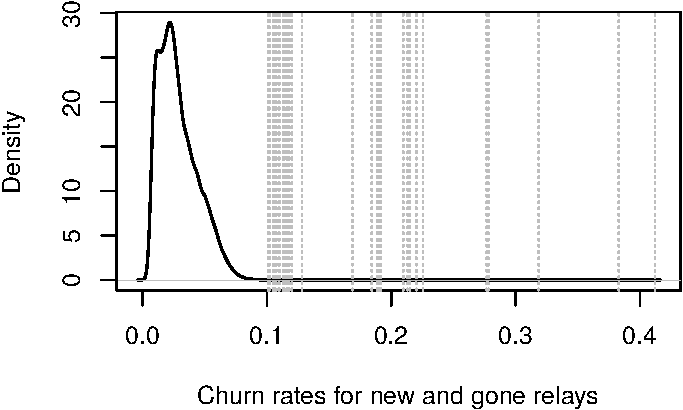
\includegraphics[width=\linewidth]{diagrams/churn-density.pdf}
	\caption{Density of all churn values for new and gone relays.  For both
	time series, 37 churn rates over eight years exceeded 0.1.  The dotted
	vertical lines mark all outliers.}
	\label{fig:churn-density}
\end{figure}

\begin{table}[t]
	\centering
	\begin{tabular}{ccccccc}
	\textbf{Churn type} & \textbf{Min.} & \textbf{Median} & \textbf{Mean} & \textbf{Max.} \\
	\hline
	New & 0.000 & 0.026 & 0.029 & 0.319 \\
	Gone & 0.003 & 0.025 & 0.029 & 0.412 \\
	\end{tabular}
	\caption{Summary of the distribution of churn rates for all consensuses
	since 2007.}
	\label{tab:churn-dist}
\end{table}

Figure~\ref{fig:2008-08} illustrates the churn rates for August 2008, featuring
our biggest anomaly.  On August 19, 822 relays left the network, resulting in a
sudden spike of the churn rate, and a trend increase in the time series.  The
spike was caused by the switch from consensus method three to four, which
happened on August 19, 2008.  The changelog says that in consensus method four,
routers that don't have the \texttt{Running} flag are no longer listed in the
consensus.

\begin{figure}[t]
	\centering
	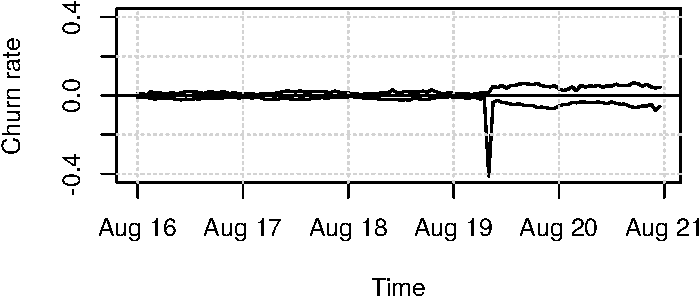
\includegraphics[width=\linewidth]{diagrams/2008-08.pdf}
	\caption{On August 19, 822 relays suddenly left the Tor network, resulting
	in a churn rate spike, and a time series increase.  The event was caused by
	the switch from consensus method three to four.}
	\label{fig:2008-08}
\end{figure}

\mynote{Still need to discuss other outliers.}

\subsection{Uptime analysis}
\label{sec:uptime}
We generated relay uptime illustrations for every month since 2007, resulting in
93 uptime visualizations.\footnote{All images are available online, on the following
onion service: \url{http://qviewr5ittnqdcvi.onion}.}
We now discuss a subset of these images that
contain particularly interesting patterns.

Figure~\ref{fig:2010-06-planetlab} shows June 2010, featuring a clear ``Sybil
block'' on the left side.  The Sybils belonged to a researcher who, as
documented by The Tor Project~\cite{progressreport}, started 512 Tor relays on
PlanetLab for research on scalability.  Our manual analysis could verify this.
The relays were easy to identify because their nicknames suggested that they
were hosted on PlanetLab, containing strings such as ``planetlab,'' ``planet,''
and ``plab.''  Note the small height of the Sybil block, indicating that the
relays were not online for a long time.

\begin{figure}[t]
	\centering
	
\includegraphics[width=\linewidth]{diagrams/planetlab-uptimes.jpg}
	\caption{In June 2010, a researcher started 512 Tor relays on PlanetLab for,
		as The Tor Project documented, ``their research into cloud computing and
		scaling effects''~\cite{progressreport}.  As illustrated by the easily
		visible red bar on the left, the relays were only online for a short
		while.}
	\label{fig:2010-06-planetlab}
\end{figure}

Figure~\ref{fig:2012-08-steppattern} features a curious ``step pattern'' for
approximately 100 relays, all of which were located in Russia and Germany.  The
relays appeared in December 2011, and started exhibiting the diurnal step
pattern (nine hours uptime followed by 15 hours downtime) in March 2012.  All
relays had similar nicknames, consisting of eight seemingly randomly-generated
characters.  In April 2013, the relays finally disappeared.

\begin{figure}[t]
	\centering
	
\includegraphics[width=\linewidth]{diagrams/2012-08.jpg}
	\caption{August 2012 featured a curious ``step pattern,'' caused by
	approximately 100 Sybils.  Out of 24 hours, the relays were online for only
	nine hours.}
	\label{fig:2012-08-steppattern}
\end{figure}

Figure~\ref{fig:2014-04-heartbleed} shows the effect of the Heartbleed
incident~\cite{Durumeric2014a} on the Tor network.  Several days after the
incident, The Tor Project decided to block all relays that haven't generated new
key pairs.  The large red block in the middle of the picture illustrates when
the biggest part of the block became active, rejecting approximately 1,700 Tor
relay fingerprints.
% $ wc -l dirauth-conf/approved-routers.d/bleeding-edges.conf
% 1779 dirauth-conf/approved-routers.d/bleeding-edges.conf

\begin{figure}[t]
	\centering
	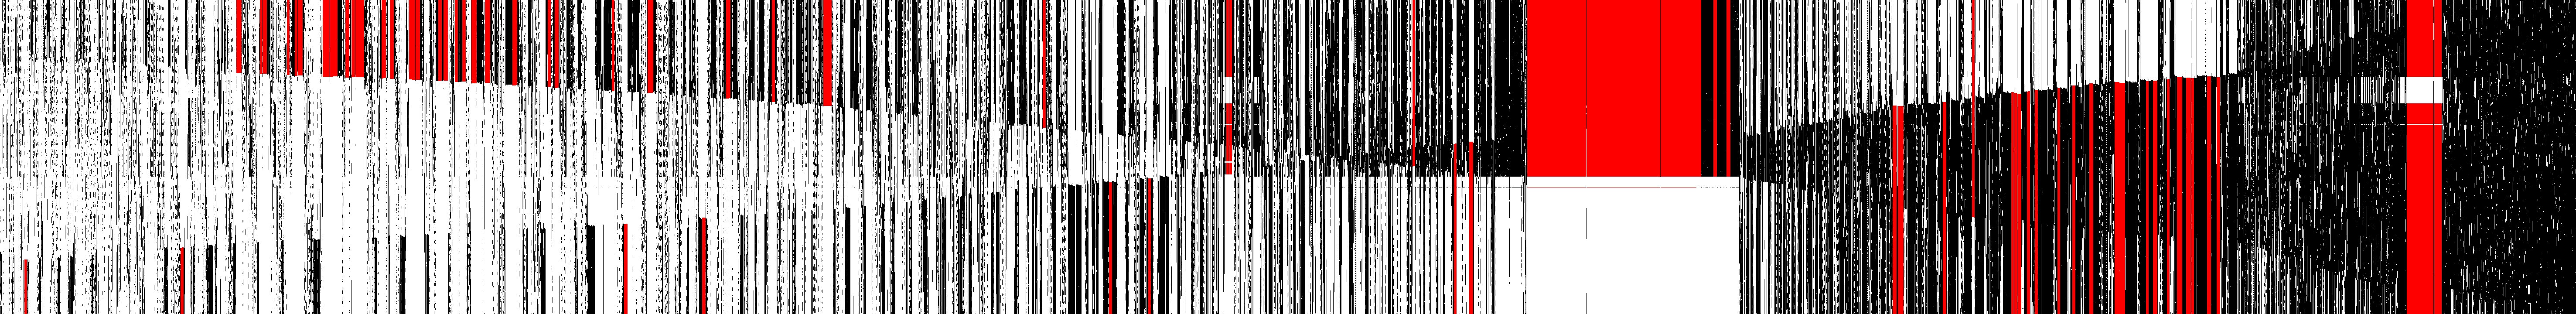
\includegraphics[width=\linewidth]{diagrams/heartbleed-uptimes.jpg}
	\caption{April 2014, the month the Heartbleed bug was discovered.
		The large block in the middle of the diagram happened because The
		Tor Project eventually rejected a large number of relays that did not
		change their keypairs in time.}
		\label{fig:2014-04-heartbleed}
\end{figure}

Figure~\ref{fig:2014-12-lizard} illustrates the largest Sybil group to date,
comprising 3,347 Tor relays that an attacker started in the Google cloud in
December 2014.  Because of its magnitude, the attack was spotted almost
instantly, and The Tor Project was quick to remove the offending relays nine
hours after the appeared.

\begin{figure}[t]
	\centering
	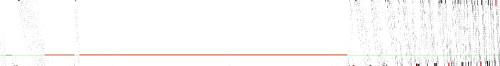
\includegraphics[width=\linewidth]{diagrams/lizard-uptimes.jpg}
	\caption{December 2014, when attackers started several hundred Tor
	relays in the Google cloud.  The relays were only online for a small number
	of hours because they were promptly rejected by The Tor Project.}
	\label{fig:2014-12-lizard}
\end{figure}

\subsection{Fingerprint anomalies}
\label{sec:fingerprint-anomalies}
We determined how often all Tor relays changed their fingerprint from 2007 to
2015.  Figure~\ref{fig:fingerprints} illustrates the amount of fingerprints
(y-axis) we have observed for the 1,000 Tor relays (x-axis) that changed their
fingerprint the most.  All these relays changed their fingerprint at least ten
times.  Twenty one relays changed their fingerprint more than 100 times, and the
relay at the very right end of the distribution changed its fingerprint 936
times.  This relay's nickname was ``openwrt,'' suggesting that it was a home
router that was rebooted regularly.  It was running from August 2010 to December
2010.

\begin{figure}[t]
	\centering
	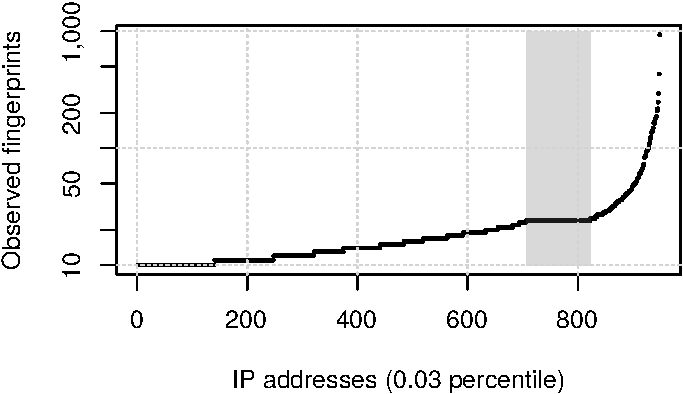
\includegraphics[width=\linewidth]{diagrams/fingerprints.pdf}
	\caption{The amount of observed fingerprints for the 1,000 relays that
	changed their fingerprints the most.  Note the curious plateau in the shaded
	area between index 707 and 803---a Sybil group that changed their
	fingerprint exactly 24 times, probably as part of an experiment for a
	S\&P'13 paper~\cite{Biryukov2013a}.}
	\label{fig:fingerprints}
\end{figure}

Figure~\ref{fig:fingerprints} further contains a peculiar plateau, shown in the
shaded area between index 707 and 803.  This plateau was caused by a group of
Sybils, hosted in Amazon EC2, that changed their fingerprint exactly 24 times.

We also found that many IP addresses in the range 199.254.238.0/24 changed their
fingerprint frequently.  We contacted the owner of the address block and were
told that the block used to host VPN services.  Apparently, several people
started Tor relays and since the VPN service would not assign permanent IP
addresses, the Tor relays would periodically change their address, causing the
churn we observe.

\subsection{Sybil characterization}
\label{sec:sybil_groups}
Table~\ref{tab:sybils} contains the Sybil groups we identified using sybilhunter
and our custom exitmap modules.  For every group, we document when we first
discovered it, its ``name,'' maximal size, and a description of its purpose.  We
now give an overview of the more interesting groups we exposed.

\begin{table*}[t]
\centering
\begin{tabular}{l c c p{10cm}}
\textbf{Discovery} & \textbf{Group ID} & \textbf{\# of relays} & \textbf{Characteristics} \\
\hline
2015-11-17 & rewrite$\dagger$ & 8 & Replaced onion domains with impersonation site. \\

2015-07-10 & DenkoNet & 58 & Hosted on Amazon AWS and only present in a single
consensus.  No relay had the \texttt{Exit} flag. \\

2015-07-02 & cloudvps & 55 & All relays only had the \texttt{Running} and
\texttt{Valid} flag.  As their name suggests, the relays were hosted by
the Dutch hoster ``CloudVPS.'' \\

2015-06-29 & rewrite$\dagger$ & 55 & Replaced onion domains with impersonation site. \\

% 2015-06-17 & 1jabberat & 12 & \ldots \\

2015-06-03 & fingerprints & 28 & All relays, located in the same /24, changed
their fingerprint regularly, presumably in an attempt to manipulate the
distributed hash table. \\

2015-04-22 & rewrite$\dagger$ & 70 & Replaced onion domains with impersonation site. \\

2015-03-11 & redirect$\ddagger$ & 24 & Redirected users to impersonated site. \\
2015-02-11 & redirect$\ddagger$ & 17 & Redirected users to impersonated site. \\
2015-01-09 & redirect$\ddagger$ & 23 & Redirected users to impersonated site. \\

2015-08 & default & --- & Likely a Windows-powered botnet.  The group
features wide, geographical distribution, which is uncommon for typical Tor
relays. \\
% Shared: nickname, IP address, port, platform, version.

2014-12-30 & Anonpoke & 284 & The relays did not have the \texttt{Exit} flag and
were removed from the network before they could get the \texttt{HSDir} flag. \\

2014-12-26 & FuslVZTOR & 246 & The relays showed up only hours after the
LizardNSA incident. \\

2014-12-26 & LizardNSA & 3,347 & A group publicly claimed to be responsible for
the attack~\cite{lizards}.  All relays were hosted in the Google cloud and The
Tor Project removed them within hours. \\

2013-02-03 & AmazonEC2 & 57 & The relays were likely part of a research
project~\cite{Biryukov2013a}. \\

2014-01-04 & FDCservers & 126 & Relays that were involved in an onion service
deanonymization attack~\cite{cmucert}. \\

2010-09-09 & trotsky & 219 & The relays could have been part of a botnet. \\

2010-06-26 & planetlab & 512 & According to a report from The Tor
Project~\cite{progressreport}, a researcher started these relays to learn more
about scalability effects. \\
\end{tabular}
\caption{The Sybil groups we discovered using sybilhunter and our custom exitmap
modules.}
\label{tab:sybils}
\end{table*}

\sybilgroup{The ``rewrite'' Sybils}
All relays had the \texttt{Exit} flag and replaced onion domains with an
impersonation, presumably hosted by the attacker.  Interestingly, the
impersonation domains shared a prefix with the original, e.g.,
\textbf{sigaint}bulkwy2vl.onion was replaced with
\textbf{sigaint}z7qjj3val.onion.  The shared prefix means that the attacker was
generating vanity domains by repeatedly generating public key pairs until the
hash over the key resembled the desired prefix.  Onion domains are generated by
determining the SHA-1 hash over the public key, truncating it to the 80 most
significant bits, and encoding it in Base32.  Each Base32 digit of the
16-digit-domain represents five bits.  As a result, to get an $n$-digit prefix
in the onion domain, $2^{5 n - 1}$ operations are required on average.  For the
seven-digit prefix above, this results in $2^{5 \cdot 7 - 1} = 2^{34}$
operations.  The author of scallion~\cite{scallion}, a tool for generating
vanity onion domains, determined that an nVidia Quadro K2000M, a mid-range
laptop GPU, is able to generate 90 million hashes per second.  On this GPU, a
partial collision for a seven-digit prefix can be found in $2^{34} \cdot
\frac{1}{90,000,000} \simeq 190$ seconds, i.e., in a little bit more than three
minutes.

We found that attacked onion domains contained Bitcoin wallet addresses that
were replaced in the impersonation, presumably to hijack donations or payments.
As a result, we believe that the attack was financially motivated.

\sybilgroup{The ``redirect'' Sybils}
The relays all had the \texttt{Exit} flag and tampered with HTTP redirects of
exit traffic.  Some Bitcoin sites would redirect users from their HTTP version
to the secure HTTPS version, to protect their users login credentials.  This
Sybil group, however, tampered with the redirect and directed users towards an
impersonation site, resembling the original Bitcoin site, perhaps to steal
credentials.  We only observed this attack for Bitcoin sites, but cannot rule
out that other sites were not attacked.

Interestingly, the Sybils' server descriptors and consensus entries had less in
common than other Sybil groups.  They used a small set of different ports, Tor
versions, bandwidth values, and their nicknames did not exhibit an
easily-recognizable pattern.  In fact, we can only clearly identify these Sybils
because of the active attack they run, using exitmap, and not because of their
appearance.

We discovered three Sybil clusters that implemented the redirect attack, each of
them surfacing when the previous one got blocked.  The first group first showed
up in May 2014, with only two relays, but slowly grew over time, until it was
finally discovered in Jan 2015.  We believe that they were run by the same
attacker because of the way the attack was implemented.

\sybilgroup{The ``default'' Sybils}
This Sybil group, named after the shared nickname ``default,'' has been around
since 2011 (see Figure~\ref{fig:default-over-time}) and consists of
Windows-powered relays only.  We extracted relays by filtering consensuses
for nicknames that are set to ``default,'' onion routing ports set to 443, and
directory ports set to 9030.  The group features high IP address churn.  For
Oct. 2015, we found ``default'' relays in 73 countries, with the top three
countries being Germany~(50\%), Russia~(8\%), and Austria~(7\%).  The majority
of these relays, however, has little uptime.
Figure~\ref{fig:default-sybils-uptime} shows the uptime matrix for ``default''
relays in Oct. 2015.  Many relays exhibit a diurnal pattern, suggesting
that they are powered off regularly---as it often is the case for desktop PCs.

\begin{figure}[t]
	\centering
	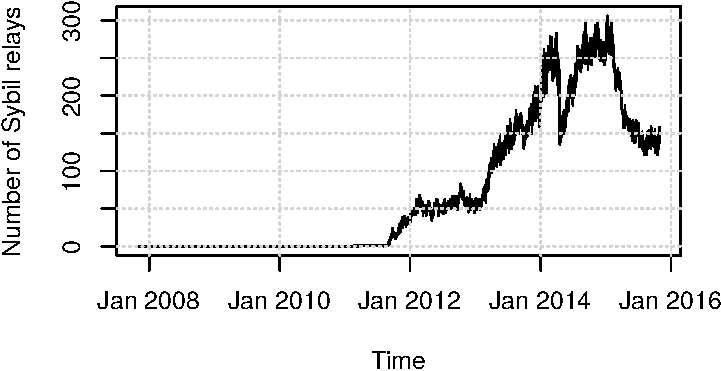
\includegraphics[width=\linewidth]{diagrams/default-over-time}
	\caption{The amount of members of the ``default'' Sybil group over time.
		The relays surfaced in Sep 2011 and occasionally amounted to several
		hundred members online at the same time.}
	\label{fig:default-over-time}
\end{figure}

To get a better understanding of the amount of ``default'' relays over time, we
analyzed all consensuses, extracting the number of relays whose nickname was
``default,'' whose onion routing port was 443, and whose directory port was
9001.  We did this for the first consensus every day and plot the result in
Figure~\ref{fig:default-over-time}.

The above suggests that some of these relays are running without the owner's
knowledge.  The relays don't fit the pattern of Sefnit (a.k.a.
Mevade)~\cite{sefnit} and Skynet~\cite{skynet}, two pieces of malware that use
an onion service as command and control server.  Nevertheless, we believe that
these are part of a botnet.

\sybilgroup{The ``trotsky'' Sybils}
Similar to the ``default'' cluster, the ``trotsky'' relays appear to be part of
a botnet.  Most of the relays' IP addresses were located in Eastern Europe, in
particular in Slovenia, Croatia, and Bosnia and Herzegovina.  The relays were
all running on Windows, in version 0.2.1.26, and listening on port 443.  Most of
the relays were configured as exits, and The Tor Project assigned some of them
the \texttt{BadExit} flag.

The first relays started appearing in Sep 2010.  Over time, there were two relay
peaks, reaching 139 (Sep 23) and 219 (Oct 3) relays.  After that, only 1--3
relays remained in the consensus.

\sybilgroup{The ``Amazon EC2'' Sybils}
The relays all used randomly-generated nicknames, consisting of 16 letters and
numbers; Tor in version 0.2.2.37; GNU/Linux; and IP addresses in Amazon's
netblock.  Every IP address changed its fingerprint 24 times, but not randomly:
the fingerprints were chosen systematically, in a small range.  For example,
relay 54.242.248.129 used fingerprints starting with the prefixes \texttt{8D},
\texttt{8E}, \texttt{8F}, and \texttt{90}.  The relays were online for 48 hours.
After 24 hours, most of the relays obtained the \texttt{HSDir} flag.

We believe that this Sybil group was run by Biryukov, Pustogarov, and Weinmann
for their paper ``Trawling for Tor Hidden Services''~\cite{Biryukov2013a}.

\sybilgroup{The ``LizardNSA'' Sybils}
All relays were hosted in the Google Cloud, and only online for nine hours,
until the directory authorities started rejecting them.  The majority of
machines were middle relays (96\%), but the attackers also started some exit
relays (4\%).  The Sybils were set up to be onion service directories, but the
relays were taken offline before they were assigned the \texttt{HSDir} flag.  If
all relays would have obtained the \texttt{HSDir} flag in time, they would have
constituted almost 50\% of all onion service directories; the median number of
onion service directories on Dec. 26 was 3,551.

\sybilgroup{The ``FuslVZTOR'' Sybils}
All machines were middle relays and hosted in 212.38.181.0/24, a VPS provider's
network in the UK.  The directory authorities started rejecting the relays five
hours after they were first seen.  The relays advertized the default bandwidth
of 1 GiB/s and used seemingly randomly determined ports.  Other than happening
in parallel to the LizardNSA attack, there is no reason to believe that both
incidents are related.

\sybilgroup{The ``Anonpoke'' Sybils}
All relays shared the nickname ``Anonpoke'' and were online for four hours until
they were rejected.  All relays were hosted by a VPS provider in the US,
Rackspace, with the curious exception of a single relay that was hosted in the
UK, and running a different Tor version.  The relays advertized the default
bandwidth of 1 GiB/s on port 9001 and 9030.  All relays were middle relays and
running as directory mirror.  All Sybils were configured to be an onion service
directory, but did not manage to get the flag in time.

\sybilgroup{The ``PlanetLab'' Sybils}
A set of relays that used a variation of the strings ``planet'', ``plab'',
``pl'', and ``planetlab'' as their nickname.  The relays' exit policy allowed
ports 6660--6667, but they did not get the \texttt{Exit} flag.  The Sybils were
online for three days and then removed by The Tor Project, as mentioned in a
blog post~\cite{progressreport}.  The blog post further says that the relays
were run by a researchers.

\sybilgroup{The ``FDCservers'' Sybils}
We believe that these Sybils were used in attempt to deanonymize onion services,
summarized by The Tor Project in a July 2014 blog post~\cite{cmucert}.  The
relays were running FreeBSD, did not have a nickname, and were located in
50.7.0.0/16 and 204.45.0.0/16.

%The relays were added to the network on .

On Jan 30, 2014, the attackers added 58 relays to the 63 existing ones, giving
them control over a total of 121 relays.

% \subsubsection{Bitcoin}
% The ones that are stealing bitcoins.
% 
% Look at blockchain and figure out how much they stole.

\subsection{Accuracy of nearest-neighbor search}
\label{sec:accuracy}
\mynote{This section is still very much work-in-progress.}
A proper evaluation of our algorithm's classification performance requires
ground truth, i.e., Sybil relays that are \emph{known} to belong together.  All
we have, however, are Sybils that we \emph{believe} belong together.  We can use
this dataset as ground truth, but the resulting performance scores are likely an
overestimate of our algorithm's true performance because we manually tuned it to
consider the features that we believe to be strong predictors.

% We can (ab)use MyFamily data as ground truth.
In addition to our Sybil dataset, relay families can serve as ground truth.  A
relay family is a set of Tor relays that is controlled by one operator, and is
configured to express this mutual relationship in the family members'
configuration file.  In a way, relay families can be seen as benign Sybils.  Tor
clients never use more than one member of a family in their path to prevent
correlation attacks.  As of Nov.  2015, there are approximately \mynote{XXX}
families in the network, ranging from only two relays to \mynote{XXX} relays.
We can evaluate our algorithm by making it find the nearest neighbours of a
family member, which, ideally, should be its family members.  Again, using
families as ground truth is very likely to overestimate results because family
operators frequently configure their relays almost identically.  At the time of
this writing, a popular relay family uses the nicknames ``AccessNow000'' to
``AccessNow009,'' uses adjacent IP addresses, and identical contact information.
We expect the operators of malicious Sybils, however, to go out of their way to
obscure the relationship between their relays.

% Concrete MyFamily experiment.
To evaluate our nearest-neighbour search, we used all relay families that were
present in the first consensus that was published in Oct. 2015.  \mynote{Quick
overview of how many families were present.} For every relay that had a mutual
family relationship, we built a vantage point tree and then searched for its $n$
nearest neighbours where $n$ is the amount of mutual family relationships.
Basically, we evaluated how good our algorithm is at finding the relatives of a
family member.  We determined the precision and recall, both in the interval
$[0,1]$ and telling us how many of the nearest neighbours are family members
(precision) and how many family members were in the nearest neighbours (recall).
More formally, precision $\mathcal{P}$ is defined as
$$\mathcal{P} = \frac{|\textrm{\footnotesize Correctly identified Sybils}|}
{|\textrm{\footnotesize Uncorrectly identified Sybils}|}$$
and recall $\mathcal{R}$ is defined as
$$\mathcal{R} = \frac{|\textrm{\footnotesize Correctly identified Sybils}|}
{|\textrm{\footnotesize Correctly identified Sybils} \cap \textrm{\footnotesize Unidentified Sybils}|}.$$
For every family member in the consensus, we determined one precision and recall
value, respectively.  All values are illustrated in
Figure~\ref{fig:precision-recall}, showing precision on the x-axis and recall on
the y-axis.  The more points in the top right corner, the better is our
algorithm's classification performance.  Most value pairs were either $(1,1)$
(XXX\%) or $(0,0)$ (YYY\%).

\begin{figure}[t]
	\centering
	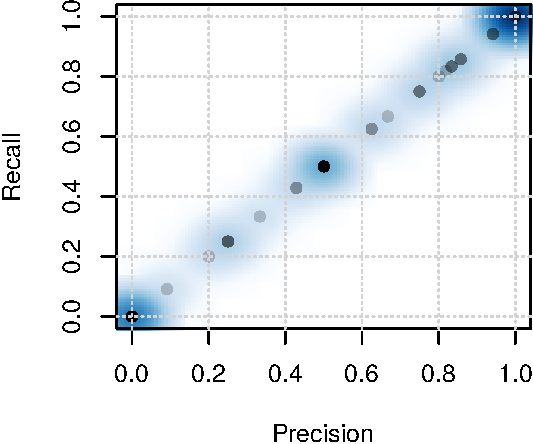
\includegraphics[width=0.32\textwidth]{diagrams/precision-recall.pdf}
	\caption{Precision and recall when our algorithm is applied on the relay
		family dataset.}
	\label{fig:precision-recall}
\end{figure}

% We manually investigated some classification results and found that
% \mynote{explain}.

\subsection{Computational cost}
\label{sec:performance}
We are interested in the computational cost of our analysis techniques.  Fast
methods lend themselves to being run hourly, for every new consensus, while
slower techniques must be run less frequent.  Table~\ref{tab:exp-deployment}
gives an overview of the runtime of our methods.\footnote{All performance
numbers were determined on an Intel Core i7-3520M CPU at 2.9 GHz, a
consumer-grade CPU.}  Note that we
placed our datasets on a solid state drive, to shift eliminate I/O as
performance bottleneck.

\begin{table}[t]
	\centering
	\begin{tabular}{lccc}
	\textbf{Method} & \textbf{Invocation} & \textbf{Analysis window} & \textbf{Run time} \\
	\hline
	Network churn & Hourly & Two consensuses & $\sim$0.16s \\
	Nearest-neighbor & Daily & One consensus & $\sim$15s \\
	Fingerprint analysis & Daily & One month & $\sim$55s \\
	Uptime matrix & Daily & One month & $\sim$67s \\
	Similarity matrix & Daily & One consensus & XXX \\
	\end{tabular}
	\caption{The computational cost of our analysis techniques, measured in
	execution time.  Network churn analysis is very fast and can easily be run
	hourly while the creation of a similarity matrix takes more time and can be
	run daily.}
	\label{tab:exp-deployment}
\end{table}

The table columns contain, from left to right, our analysis technique, how often
we intend to run the technique, the technique's data time window, and how long
it takes to compute its output.  The calculation of network churn is very
fast---it takes as input only two consensus files---and can easily be done for
every network consensus.  Nearest-neighbour search takes approximately 15
seconds, most of which is spent building the vantage point tree.  We used
nearest-neighbour search for manual analysis, but it can also be used
automatically.  Fingerprint and uptime analysis for one month work of consensus
files both take approximately one minute and can easily be run daily.
%Finally, computing a similarity matrix takes \mynote{XXX}.
